\emph
{
            Ejecute y explique la funci\'on del siguiente c\'odigo en Octave. Comente qu\'e 
            teoremas del curso (y del curso de probabilidad) son importantes para interpretar 
            la figura.
            \tiny
            \texttt
            {
                \lstinputlisting[caption=]{tarea3/problema3_4/polya2.R}
            }
            \normalsize
}

\afterstatement\par\null

\begin{center}
    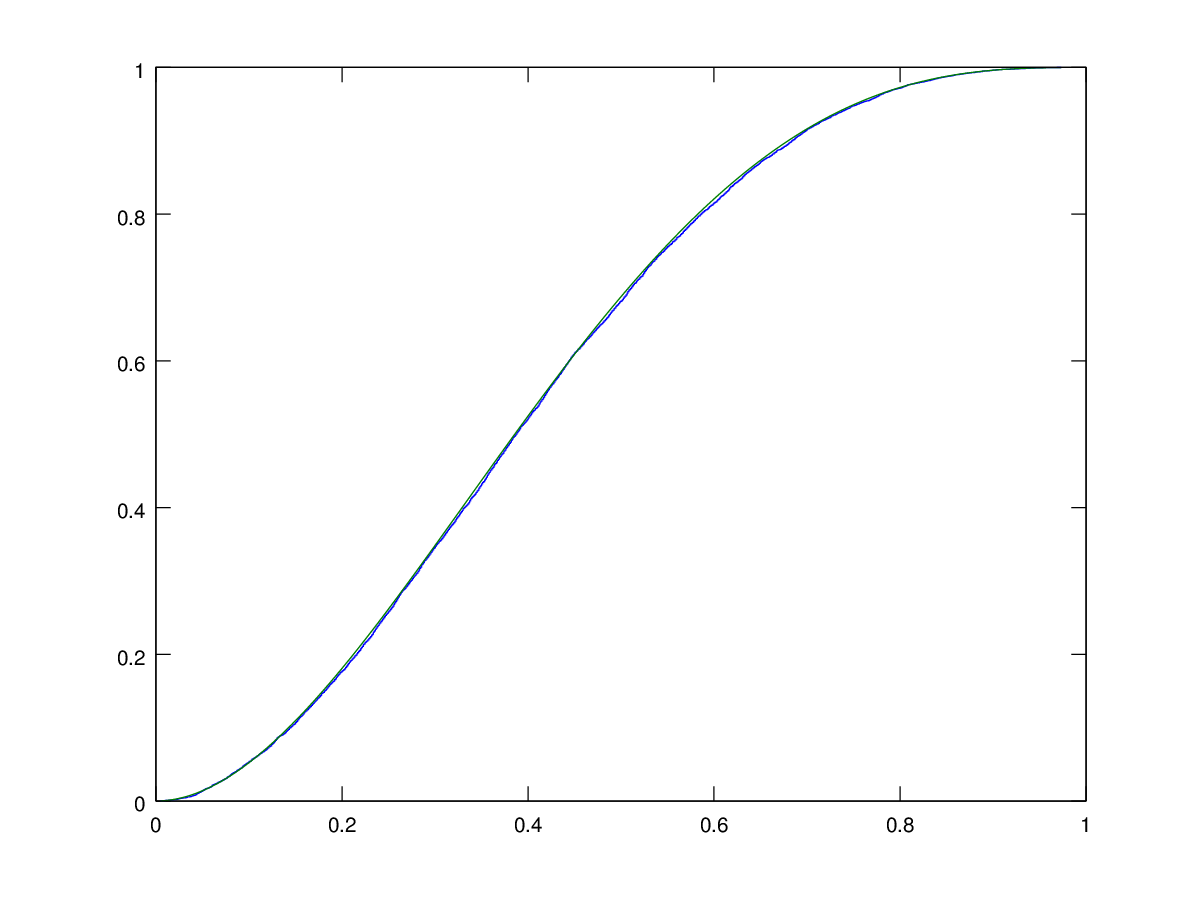
\includegraphics[width=8cm]{tarea3/problema3_4/poylaBeta.PNG}\par\null
    Gr\'afica del histagrama de los radios ``finales'' de muchas iteraciones del proceso 
	de urnas de Poyla.
\end{center}